\documentclass[12pt]{article}
\usepackage{amsmath}
\usepackage{amssymb}
\usepackage{graphicx}
\usepackage{hyperref}
\usepackage{cleveref}
\usepackage[most]{tcolorbox}
\usepackage[utf8]{inputenc}
\usepackage{tikz}
\usepackage{pstricks-add}
\usepackage{enumerate}
\usepackage{MnSymbol}
\usepackage{mathtools}
\usepackage{subcaption}
\usepackage{geometry}
 \geometry{
 a4paper,
 total={170mm,257mm},
 left=20mm,
 top=20mm,
 }
\DeclarePairedDelimiter\ceil{\lceil}{\rceil}
\DeclarePairedDelimiter\floor{\lfloor}{\rfloor}
\DeclarePairedDelimiter\abs{\left|}{\right|}
\hypersetup{
    colorlinks=false,
    pdfborder={0 0 0},
}
\newcommand\tab[1][1cm]{\hspace*{#1}}
\newtheorem{theorem}{Theorem}
\usetikzlibrary{arrows,calc}
\title{MAT 1001: Calculus I}
\author{Alfonsus Rodriques Rendy}
\date{2021-9-16}

\begin{document}
\begin{center}
    \hspace*{-0.5cm}
    \framebox{
    \begin{minipage}{1\linewidth}
        \textbf{MAT1001 Calculus I} \\
        \vspace{-0.8cm}
        \begin{center}
            \huge{Lecture 4 - 7 : Derivatives} 
            \\
            \vspace{0.5cm}
            \normalsize \textit{Lecture by Dr. Arjan Abeynaike} \\
            \vspace{0.3cm}
            \text{Scribe by Alfonsus Rodriques Rendy} \\
            \textrm{Sep 16, 2021 - Sep 30, 2021}
        \end{center}
    \end{minipage}}
\end{center}

\section{Derivatives}
\subsection{Definition}
\paragraph{Definition: Interior Point} Let $S \subseteq \mathbb{R}$ A point $c \in S$ is called an \textbf{interior point} of $S$ 
if there exists $a > 0$ such that
\[
    (c - a, c + a) \subseteq S
\]

\begin{figure}[h!]
    \centering
    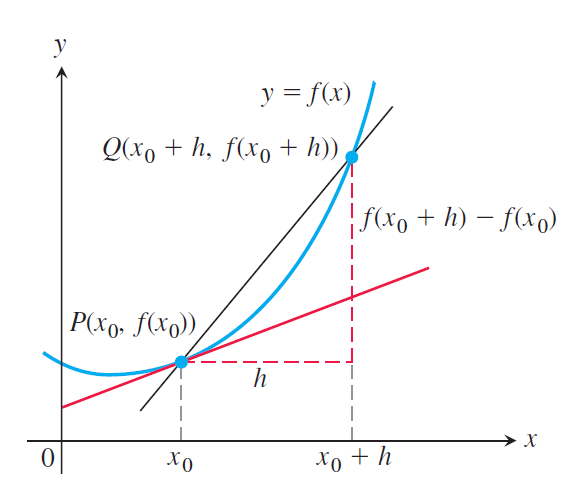
\includegraphics[width = 0.45\linewidth]{Images/derivative.png}
    \caption{The slope of the tangent line at $P$ is the derivative of $f(x)$ at P}
\end{figure}

\paragraph{Definition}Let $f : D \to \mathbb{R}$ be a function and let $x_0$ be an interior point of $D$. Then 
the derivative of $f$ at $x_0$, denoted by $f'(x_0)$, is defined by
\[
    f'(x_0) = \lim_{h \to 0} \frac{f(x + h) - f(x)}{h} = \lim_{x \to x_0} \frac{f(x) - f(x_0)}{x - x_0} 
\]
Provided that the limit exists. \\

\noindent
For $y = f(x)$, $f'(x_0)$ can be represented as:
\begin{itemize} 
     \item The slope of the tangent line of the graph $f(x)$ at $x = x_0$
     \item The instantaneous rate of change of y w. r. t. x at $x = x_0$
\end{itemize}

\paragraph{Notations} There are many ways to denote the derivative of $y = f(x)$. Some notations are:
\[
    f'(x) = y' = \frac{dy}{dx} = \frac{df}{dx} = \frac{dy}{dx} f(x) = D(f)(x) = D_x f(x) 
\]
We read $dy/dx$ as “the derivative of $y$ with respect to $x$,” and $df/dx$ and $(dy/dx) f(x)$ as “the derivative of $f$
with respect to $x$.” The “prime” notations $y'$ and $f'$ come from notations that Newton
used for derivatives. The $dy/dx$ notations are similar to those used by Leibniz. 
\subsection{One-Sided Derivative}
Since the definition on previous section is for interior point, it can't be applied for
endpoints. For endpoints we have one-sided derivative.

\begin{figure}[h!]
    \centering
    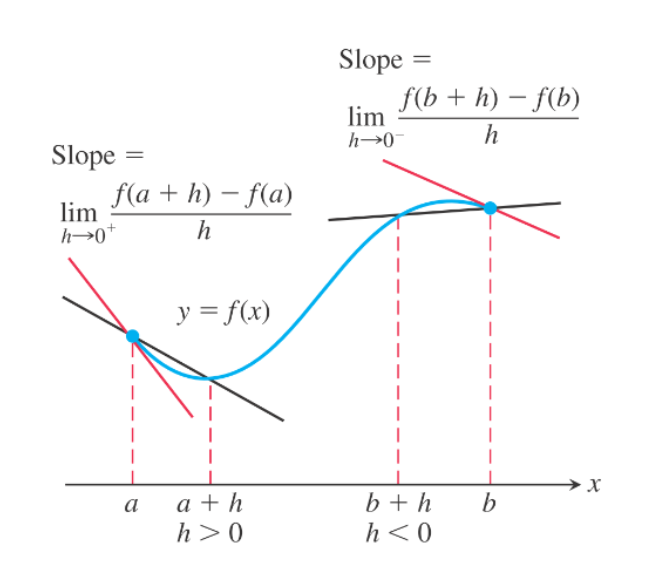
\includegraphics[width = 0.5\linewidth]{Images/derivative endpoints.png}
    \caption{Derivatives of endpoints of a closed interval}
\end{figure}

\paragraph{Definition: Right-hand Derivative}
$f : [a, b] \to \mathbb{R}$ be a function.  For each $x \in [a, b)$, \textbf{the right-hand derivative} of $f$ at $x_0$, 
denoted by $f^{'}_{+}(x_0)$, is defined by
\[
    f^{'}_{+}(x_0) = \lim_{h \to 0^{+}} \frac{f(x + h) - f(x)}{h} = \lim_{x \to x_0^{+}} \frac{f(x) - f(x_0)}{x - x_0} 
\]

\paragraph{Definition: Left-hand Derivative}
$f : [a, b] \to \mathbb{R}$ be a function.  For each $x \in (a, b]$, \textbf{the left-hand derivative} of $f$ at $x_0$, 
denoted by $f^{'}_{-}(x_0)$, is defined by
\[
    f^{'}_{-}(x_0) = \lim_{h \to 0^{-}} \frac{f(x + h) - f(x)}{h} = \lim_{x \to x_0^{-}} \frac{f(x) - f(x_0)}{x - x_0} 
\]

\subsection{Differentiability}
\paragraph{Definition}
A function $y = f(x)$ is differentiable on an open interval (finite or infinite) if it has a
derivative at each point of the interval. It is differentiable on a closed interval $[a, b]$ if it
is differentiable on the interior $(a, b)$ and if the right-hand derivative at $a$ and left-hand derivative at $b$ exists at endpoints.

\begin{theorem}[Differentiability implies continuity]
    If $f$ is differentiable at $c$, then $f$ is continuous at $c$.
\end{theorem}

\paragraph{Proof} Given that $f'(c)$ exists, we need to show that $\lim_{x \to c} f(x) = f(c)$ 

\begin{align*} 
    \lim_{x \to c} f(x) - f(c) &= \lim_{x \to c} f(x) - \lim_{x \to c} f(c) \\
    &= \lim_{x \to c} f(x) - f(c) \\
    &= \lim_{x \to c} \frac{f(x) - f(c)}{x - c} \cdot (x - c) \\
    &= \lim_{x \to c} \frac{f(x) - f(c)}{x - c} \cdot \lim_{x \to c} (x - c) \\
    &= f'(c) \cdot 0 \\
    &= 0
\end{align*}
Hence, we have
\begin{align*} 
    \lim_{x \to c} f(x) - f(c) = 0 \\
    \lim_{x \to c} f(x) = f(c)
\end{align*}

\noindent
Note that, the converse of the statement is not true, that is
\[
    f \textrm{ continuous at } c \nRightarrow f \textrm{ differentiable at } c
\]
\paragraph{Example 1} $f(x) = |x|$ is continuous but not differentiable at 0
\paragraph{Example 2} Show that
\[ f(x) =
    \begin{cases} 
        x \sin{\frac{1}{x}} & x \neq 0 \\
        0 & x = 0 \\
    \end{cases}
\]
is continuous but not differentiable at 0! \\

\noindent
To check whether $f(x)$ is continuous at 0, we need to show that $\lim_{x \to c} f(x)$ exists. Since 
$\sin{1/x}$ is a bounded function and $\lim_{x \to 0} x$ = 0 then, 
\[
    \lim_{x \to 0} x \sin{\frac{1}{x}} = 0
\]

\noindent
To check whether $f(x)$ is differentiable at 0, we need to show that $\lim_{h \to 0} \frac{f(0 + h) - f(0)}{h}$ exists. 
\begin{align*} 
    \lim_{h \to 0} \frac{f(0 + h) - f(0)}{h} &= \frac{f(h)}{{h}} \\
    &= \lim_{h \to 0} \sin{\frac{1}{h}} \\
    &= \textrm{Does Not Exist}
\end{align*}

\noindent
Hence, $f(x)$ is continuous but not differentiable at 0.

\paragraph{Non-Differentiability} There are some cases that a function is not differentiable at a points, such as:
\begin{itemize} 
     \item Corner: where the one-sided derivatives differ  ($f^{'}_{-}(x) \neq f^{'}_{+}(x)$)
     \item Cusp : where the slope approaches $\infty$ from one side and $-\infty$ from the other side
     \item Vertical tangent : where the slope approaches either $\infty$ or $-\infty$from both sides.
     \item Discontinuity : where the function is not continuous at a point
\end{itemize}

\begin{figure}[h!]
    \centering
    \begin{subfigure}{0.4\linewidth}
        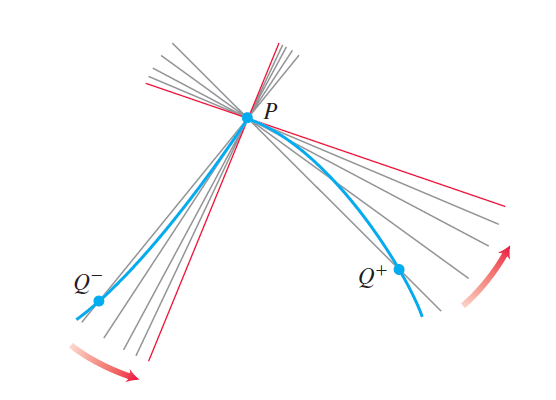
\includegraphics[width = 0.8\linewidth]{Images/corner.png}
        \caption{corner}
    \end{subfigure}
    \begin{subfigure}{0.3\linewidth}
        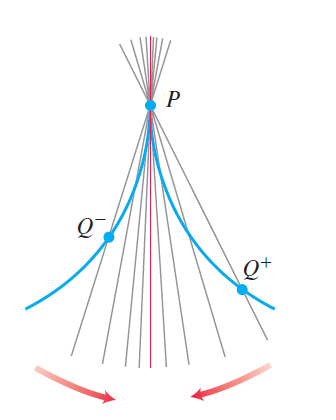
\includegraphics[width = 0.8\linewidth]{Images/cusp.png}
        \caption{cusp}
    \end{subfigure}
    \begin{subfigure}{0.3\linewidth}
        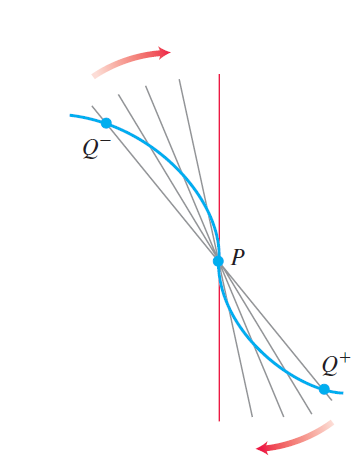
\includegraphics[width = 0.8\linewidth]{Images/vertical tangent.png}
        \caption{vertical tangent}
    \end{subfigure}
    \begin{subfigure}{0.6\linewidth}
        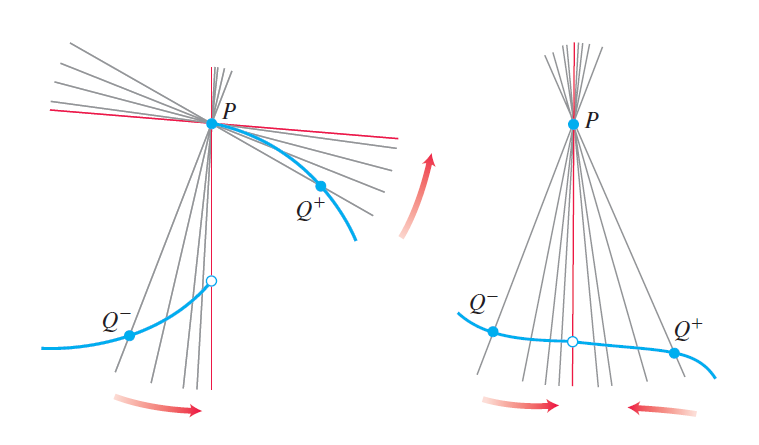
\includegraphics[width = 0.8\linewidth]{Images/discontinue.png}
        \caption{Discontinuity}
    \end{subfigure}
    \caption{Non-differentiability}
\end{figure}

\section{Differentiation Rules}
\subsection{Constant Function}
If $f(x) = c$ is a constant function, then $f'(x) = 0 \textrm{,  } \forall x \in D$
\subsection{Rule of Linearity}
The derivative of any linear combination of functions equals the same linear combination of the derivatives of the functions. \\
For any constants $\alpha$, $\beta \in \mathbb{R}$
\[
    (\alpha f(x) + \beta g(x))' = \alpha f'(x) + \beta g'(x)
\]
Linearity implied several rules:
\paragraph{Scalar Multiplication} $(\alpha f(x))' = \alpha f'(x)$
\paragraph{Addition Rule} $(f(x) + g(x))' = f'(x) + g'(x)$
\paragraph{Difference Rule} $(f(x) + g(x))' = f'(x) - g'(x)$

\subsection{Power Rule}
Let $f(x) = x^n$, where $n \in \mathbb{R}$ is a constant. Then
\[
    f'(x) = n x^{n - 1}
\]
for all $x$ where $x^n$ and $x^{n-1}$ are defined.

\paragraph{Proof} Let $f(x) = x^n$, then
\[
    f'(x) = \lim_{h \to 0} \frac{(x + h)^n - x^n}{h} 
\]
From binomial expansion, we have
\begin{align*} 
    (x + h)^n &= x^n + nx^{n - 1}h + \dots + + h^n \\
    &= x^n + nx^{n - 1}h + O(h^2)
\end{align*}
*$O(h^2)$ means all elements that contain $h^n$ with $n >= 2$. \\
\noindent
So, 
\begin{align*} 
    f'(x) = \lim_{h \to 0} \frac{(x + h)^n - x^n}{h} &= \lim_{h \to 0} \frac{x^n + nx^{n - 1}h + O(h^2)- x^n}{h} \\
    &= \lim_{h \to 0} \frac{nx^{n - 1}h + O(h^2)}{h} \\
    &= nx^{n - 1} + 0 \\
    &= nx^{n - 1} 
\end{align*}

\subsection{Product Rule}
if $f$ and $g$ are differentiable at $x$, then
\[
    (f \cdot g (x))' = f(x)g'(x) + g(x)f'(x)
\]

\paragraph{Intuitive Proof}

\begin{figure}[h!]
    \centering
    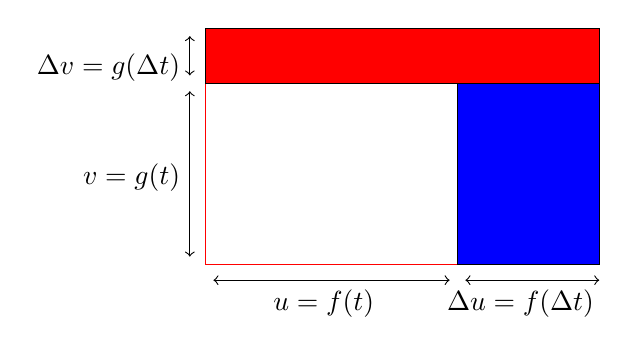
\begin{tikzpicture} 
        \draw[draw=black] (0,0) rectangle ++(5,3);
        \draw[draw=red] (0,0) rectangle ++(3.2,2.3);
        \draw[draw=black, <->] (-0.2, 0.1) -- (-0.2, 2.2) node[left, yshift=-1.1cm] {$v = g(t)$};
        \draw[draw=black, <->] (0.1, -0.2) -- (3.1, -0.2) node[below, xshift=-1.6cm] {$u = f(t)$};
        \draw[draw=black, <->] (-0.2, 2.4) -- (-0.2, 2.9) node[left, yshift=-0.4cm] {$\Delta v = g(\Delta t)$};
        \draw[draw=black, <->] (3.3, -0.2) -- (5, -0.2) node[below, xshift=-1cm] {$\Delta u = f(\Delta t)$};
        \draw[fill=red] (0,2.3) rectangle ++(5,0.7);
        \draw[fill=blue] (3.2,0) rectangle ++(1.8,2.3);
    \end{tikzpicture}
\end{figure}

Let $u = f(t)$ and $v = g(t)$. From the figure we can see that:
\begin{align*} 
     \textrm{Area of red } = f(t + \Delta t) \cdot g(\Delta t) = f(t + \Delta t) \cdot \Delta v\\
     \textrm{Area of blue } = g(t) \cdot f(\Delta t) = g(t) \cdot \Delta u
\end{align*}
Then, we can find the changes of area $\Delta uv$ :
\begin{align*} 
    \Delta (uv) &= (f \cdot g)(t + \Delta t) - (f \cdot g)(t) \\
    &= f(t + \Delta t) \Delta v + g(t) \Delta u 
\end{align*}
If we divide by $\Delta t$, we have:
\begin{align*} 
    \frac{\Delta (uv)}{\Delta t} &= f(t + \Delta t) \frac{\Delta v}{\Delta t}  + g(t) \frac{\Delta u}{\Delta t} \\
\end{align*}
From the definition:
\begin{align*} 
    \frac{d}{dt} uv = \lim_{\Delta t \to 0} \frac{\Delta (uv)}{\Delta t} &= \lim_{\Delta t \to 0} f(t + \Delta t) \frac{\Delta v}{\Delta t}  + g(t) \frac{\Delta u}{\Delta t} \\
    &= \left[\lim_{\Delta t \to 0} f(t + \Delta t) \right] \left[\lim_{\Delta t \to 0} \frac{\Delta v}{\Delta t} \right]  + g(t) \left[\lim_{\Delta t \to 0} \frac{\Delta u}{\Delta t} \right]\\
    &= f(t)g'(t) + g(t)f'(t)
\end{align*}

\subsection{Quotient Rule}
if $f$ and $g$ are differentiable at $x$ and $g(x) \neq 0$, then
\[
    \left(\frac{f(x)}{g(x)} \right)' = \frac{f'(x)g(x) - g'(x)f(x)}{g(x)^2} 
\]
\paragraph{Note} For formal proofs for all differentiation rules, see Chapter 3.3 of Thomas Calculus.

\section{Higher Order Derivative}
\paragraph{Definition} Let $f : D \to \mathbb{R}$ be a function.
\begin{itemize} 
    \item if $f'$ is differentiable at $c$ then we call $f''(x)$ the second derivative of $f$ at $c$, which we denote by $f''(c)$ or $f^{(2)} (c)$.
    \item if $f''$ is differentiable at $c$ then we call $f'''(x)$ the third derivative of $f$ at $c$, which we denote by $f'''(c)$ or $f^{(3)} (c)$.
    \item Generally, we can define the \textbf{$n^{th}$ derivative} of $f$ at $c$ to be $(f^{(n-1)})'(c)$ which we denote by $f^{(n)} (c)$.
\end{itemize}

\paragraph{Notation} The notation of higher order derivative are:
\[
    y^{(n)} = f^{(n)} = \frac{d^n}{dx^n} y = \frac{d^n y}{dx^n}
\]
Example: the notation of second derivative are
\[
    y' = f' = \frac{d^2}{dx^2} y = \frac{d^2 y}{dx^2}
\]

\section{Application of Derivative}
\subsection{Mechanics}
Suppose an object is moving. Its position is denoted as $s = f(t)$ at time $t$.

\paragraph{Definition} 
\[\]
The \textbf{displacement} of the object over a time interval $[a, b]$ is 
\[
    d = f(b) - f(a)
\]

The \textbf{instantaneous velocity} of the object at time t  is the derivative of position w.r.t time, we write as 
\[
    v(t) = \frac{ds}{dt} = \lim_{\Delta t \to 0} \frac{f(t +\Delta t) - f(t)}{\Delta t} 
\]

The \textbf{speed} of the object at time t  is absolute value of the velocity.
\[
    Speed = |v(t)| = \left| \frac{ds}{dt} \right|
\]

The \textbf{acceleration} of the object at time t  is the derivative of velocity w.r.t time, we write as 
\[
    v(t) = \frac{dv}{dt} = \frac{d^2 s}{dt^2} 
\]

The \textbf{jerk} of the object at time t  is the derivative of acceleration w.r.t time, we write as 
\[
    v(t) = \frac{da}{dt} = \frac{d^3 s}{dt^3} 
\]

\noindent
When the velocity is (+) , the object moves forward. When the velocity is (-) ,the object moves backward.
Meanwhile the speed is always positive.\\
When the acceleration is (+) , the object is speeding up (the velocity increases). When the acceleration is (-) ,
the object is slowing down (the velocity decreases)

\subsection{Cost and Production}
Suppose the cost of producing $x$ units of good is $c(x)$.
Then the marginal cost of production is the derivative of cost
w.r.t. production.
\[
    \textrm{marginal cost at $x_0$ unit of production} = c'(x_0) = \lim_{h \to 0} \frac{c(x_0 +h ) - c(x_0)}{h} 
\]

\noindent
or we can say "the cost needed to produce one more unit".

\section{Special Derivatives}
\subsection{Trigonometric Function}
The derivative of $\sin x$ and $\cos x$ are
\[
    \frac{d}{dx} \sin x = \cos x \textrm{\tab \tab}  \frac{d}{dx} \cos x = - \sin x
\]

\paragraph{Proof of the derivative of sin x} First, from the definition,
\[
    \frac{d}{dx} \sin x = \lim_{h \to 0} \frac{\sin (x + h) - \sin (x)}{h} 
\]

\noindent
From the trigonometry identity we have
\[
    \sin (x + h) = \sin x \cos h + \sin h \cos x
\]
\noindent
So,
\begin{align*} 
    \lim_{h \to 0} \frac{\sin (x + h) - \sin (x)}{h} &= \lim_{h \to 0} \frac{ \sin x \cos h + \sin h \cos x - \sin (x)}{h} \\
    &= \lim_{h \to 0} \frac{\sin h \cos x}{h} +  \lim_{h \to 0} \frac{ \sin x \cos h - \sin (x)}{h} \\
    &= \cos x \cdot \lim_{h \to 0} \frac{\sin h}{h} + \sin x  \cdot \lim_{h \to 0} \frac{ \cos h - 1}{h} \\ 
    &= \cos x \cdot 1 + \sin x \cdot 0 \\
    &= \cos x
\end{align*}

\noindent
We can also proof the derivative of $\cos x$ in the same manner but with the identity
\[
    \cos (x + h) = \cos x \cos h - \sin x \sin h
\]
\\
\noindent
The derivative of $\tan x$ is 
\[
    \frac{d}{dx} \tan x = \sec^2 x
\]
\paragraph{Proof of the derivative of tan x} We know that
\[
    \tan x = \frac{\sin x}{\cos x} 
\]
So, by using quotient rules
\begin{align*} 
    \frac{d}{dx} \tan x = \frac{d}{dx} \frac{\sin x}{\cos x} &= \frac{ \frac{d}{dx} \sin x \cdot \cos x - \frac{d}{dx}\cos x * \sin x}{\cos^2 x} \\
    &= \frac{\cos^2 x + \sin^2 x}{\cos^2 x} \\
    &= \frac{1}{\cos^2 x}\\
    &= \sec^2 x
\end{align*}

The derivative of other trigonometric functions are:
\begin{align*} 
    &\frac{d}{dx} \sec x = \sec x \tan x \textrm{\tab \tab} &&\frac{d}{dx} \csc x = - \csc x \cot x \\
    &\frac{d}{dx} \tan x = \sec^2 x &&\frac{d}{dx} \cot x = - \csc^2 x
\end{align*}

\subsection{Natural Exponential Function}
\subsubsection{Euler Constant}
Suppose we have 1 USD. You put in in a bank with annual interest of 100 percent. Interest is compounded $n$ times a year. 
So, we have:
\[
    \textrm{Return Value } = \left(1 + \frac{1}{n} \right)^n
\]
As we increase n, the return value gets closer to the number, the euler constant denoted by $e$, where
$e \approx 2.71828...$

\paragraph{Definition}
The euler constant $e$ is defined by 
\[
    e = \lim_{x \to \infty} \left( 1 + \frac{1}{x} \right)^x
\]

\noindent
We also have:
\[
    e = \lim_{x \to 0} (1 + x)^{\frac{1}{x}}
\]

\paragraph{Proof:} To proof that $\lim_{x \to 0} (1 + x)^{\frac{1}{x}} = e$, We need to show that 
\[ 
    \lim_{x \to 0^{-}} (1 + x)^{\frac{1}{x}} = \lim_{x \to 0^{+}} (1 + x)^{\frac{1}{x}} = e
\]
\noindent
Let $x = 1/y$, so as $x \to \infty$, $y \to 0^{+}$. We have
\begin{align*} 
    \lim_{x \to \infty} \left( 1 + \frac{1}{x} \right)^x = \lim_{y \to 0^{+}} \left( 1 + y \right)^{\frac{1}{y}} = e
\end{align*}

\noindent
Let $z$ satisfy
\[
    1 + y = \frac{1}{1 + z} \textrm{\tab} \forall z \in [ - 1, 0]
\]
Then
\begin{align*} 
    y = \frac{1}{1 + z} - 1 = - \frac{z}{1 + z} \textrm{\tab} \Rightarrow \textrm{\tab} \frac{1}{y} = - \frac{1 + z}{z} \\
\end{align*}

\noindent
So,
\begin{align*} 
    (1 + y)^{\frac{1}{y}} &= \left(\frac{1}{1 + z} \right)^{ -\frac{1 + z}{z}} \\
    &= (1 + z)^{\frac{1 + z}{z}} \\
    &= (1 + z)^{\frac{1}{z}}(1 + z)
\end{align*}

\noindent
As $y \to 0^{-}$, $z = \frac{-y}{1 + y} \to 0^{+}$, So
\begin{align*} 
    \lim_{y \to 0^{-}} &= \lim_{z \to 0^{+}} (1 + z)^{\frac{1}{z}}(1 + z) \\
    &= \lim_{z \to 0^{+}} (1 + z)^{\frac{1}{z}} \cdot \lim_{z \to 0^{+}} (1 + z) \\
    &= e \cdot 1 = e
\end{align*}

\paragraph{Compund Interest} 
\begin{align*} 
    P &\approx \lim_{n \to \infty} P_0 \left( 1 + r \frac{1}{n}\right)^{nt} \\
    &\approx P_0 \left[\lim_{n \to \infty} \left( 1 + \frac{1}{n/r}\right)^{\frac{n}{r}} \right]^{rt} \\
    &\approx P_0 e^{rt}
\end{align*}

\subsubsection{Derivative of $e^x$}
Let $f(x) = e^x$, then $f'(x) = e^x$.
\paragraph{Proof} First we define natural logarithm function as 
\[
    y = e^x \Rightarrow \ln y = x    
\]

\noindent 
We have special limit forms:
\[
    \lim_{x \to 0} \frac{\ln(1 + x)}{x} = 1 \textrm{\tab and \tab} \lim_{x \to 0} \frac{e^x - 1}{x} = 1 
\]

(1)
\begin{align*} 
    \lim_{x \to 0} \frac{\ln(1 + x)}{x} &= \lim_{x \to 0} \frac{1}{x} \cdot {\ln(1 + x)} \\
    &= \lim_{x \to 0} \ln(1 + x)^{\frac{1}{x}} \\
    &= \ln(\lim_{x \to 0} (1 + x)^\frac{1}{x}) \\
    &= \ln(e) = 1
\end{align*}

(2)
\\


Let $y = e^x - 1 \Rightarrow  x = \ln(1 + y)$ and as $x \to 0$, $y \to 0$
\begin{align*} 
    \lim_{x \to 0} \frac{e^x - 1}{x} &= \lim_{y \to 0} \frac{y}{\ln(1 + y)} \\
    &= \frac{1}{\lim_{y \to 0} \frac{\ln(1 + y)}{y}} = 1
\end{align*}

$f(x) = e^x$, 
\begin{align*} 
     f'(x) &= \lim_{h \to 0} \frac{e^{x + h} - e^x}{h} \\
    &= e^x \cdot \lim_{h \to 0} \frac{e^h - 1}{h} \\
    &= e^x \cdot 1 = e^x
\end{align*}

\section{Chain Rule}
\subsection{Definition}
Suppose we have three variables $x, y, z$, related by functions
$y = f(x)$, $z = g(y)$, so $z = g(f(x))$. Then we what is $dz/dx$?

\paragraph{Intuition} We have three different number lines representing each of the variables.
\begin{figure}[h!] 
    \centering
    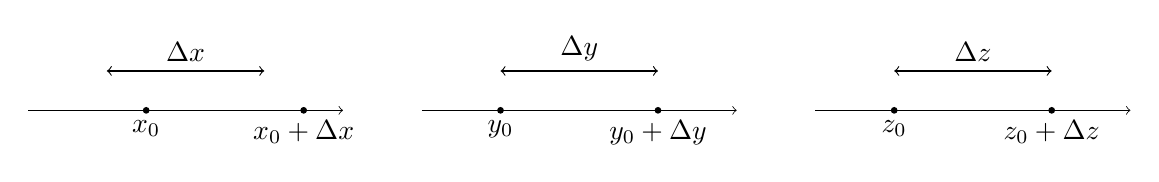
\begin{tikzpicture} 
        \draw[line width=0.1mm, draw=black, ->] (0, 0) -- (4, 0);
        \draw[draw=black, <->] (1,0.5) -- (3,0.5) node[above, xshift=-1cm] {$\Delta x$};
        \filldraw[black] (1.5,0) circle (1pt) node[below] {$x_0$};
        \filldraw[black] (3.5,0) circle (1pt) node[below] {$x_0 + \Delta x$};

        \draw[line width=0.1mm, draw=black, ->] (5, 0) -- (9, 0);
        \draw[draw=black, <->] (6,0.5) -- (8,0.5) node[above, xshift=-1cm] {$\Delta y$};
        \filldraw[black] (6,0) circle (1pt) node[below] {$y_0$};
        \filldraw[black] (8,0) circle (1pt) node[below] {$y_0 + \Delta y$};

        \draw[line width=0.1mm, draw=black, ->] (10, 0) -- (14, 0);
        \draw[draw=black, <->] (11,0.5) -- (13,0.5) node[above, xshift=-1cm] {$\Delta z$};
        \filldraw[black] (11,0) circle (1pt) node[below] {$z_0$};
        \filldraw[black] (13,0) circle (1pt) node[below] {$z_0 + \Delta z$};
    \end{tikzpicture}
\end{figure}

\noindent
First fix $x =x_0$. When $\Delta x \approx 0 $, we have
\[
    \frac{\Delta y}{\Delta x} \approx \lim_{\Delta x \to 0} \frac{\Delta y}{\Delta x} = \left. \frac{dy}{dx} \right|_{x = x_0}
\]
So, $\Delta y \approx f'(x_0) \cdot \Delta x$.

Then, when $\Delta y \approx 0 $, we have
\[
    \frac{\Delta z}{\Delta y} \approx \lim_{\Delta y \to 0} \frac{\Delta z}{\Delta y} = \left. \frac{dz}{dy} \right|_{y = y_0}
\]
So, 
\begin{align*} 
    \Delta z \approx g'(y_0) \cdot \Delta y = g'(f(x_0)) \cdot f'(x) \cdot \Delta x \\
    \frac{\Delta z}{\Delta x} \approx g'(f(x_0)) \cdot f'(x)
\end{align*}

\begin{theorem}[The Chain Rule]
    If $f(u)$ is differentiable at the point $u = g(x)$ and $g(x)$ is differetiable at x, then
    the composite function $(f \circ g)(x) = f(g(x))$ is differentiable at x, and
    \[
        (f \circ g)'(x) = f'(g(x)) \cdot g'(x)
    \]
\end{theorem}

\paragraph{Example} Position of an object at time $T$ is
\[
    s = \cos (t^2 + 1)
\]
Find the velocity!

\begin{align*} 
    v = \frac{ds}{dt} &= \frac{d}{dt} \cos (t^2 + 1) \\
    &= - \sin (t^2 + 1) \cdot \frac{d}{dx} t^2 + 1 \\
    &= - 2t \sin (t^2 + 1)
\end{align*}
\paragraph{Proving Quotient Rule Using Chain Rule} Let $ u = f(x)/g(x)$, then
\begin{align*} 
     \frac{du}{dx} &= \frac{d}{dx} \frac{f(x)}{g(x)}\\
     &= \frac{d}{dx} f(x) \cdot \frac{1}{g(x)} \\ 
     &= f(x) \cdot \frac{d}{dx} \frac{1}{g(x)} + f'(x) \cdot \frac{1}{g(x)} \\
     &= f(x) \cdot \left( - \frac{1}{g(x)^2} \right) \cdot g'(x) + f'(x) \cdot \frac{1}{g(x)} \\
     &= \frac{ - f(x) \cdot g'(x)}{g(x)^2} + \frac{f'(x) \cdot g(x)}{g(x)^2} \\
     &= \frac{f'(x) \cdot g(x) - g'(x)f(x)}{g(x)^2}
\end{align*}

\subsection{Related Rates}
We have from chain rule:
\[
    \frac{dz}{dx} = \frac{dz}{dy} \cdot \frac{dy}{dx} 
\]
\paragraph{Example 1}
Water runs into a conical tank at the rate of 0.25 $m^3$/min.
The tank stands point down and has a height of 3 m and a base radius of
1.5 m. How fast is the water level rising when the water is 1.8 m deep?

\begin{figure}[h!] 
    \centering
    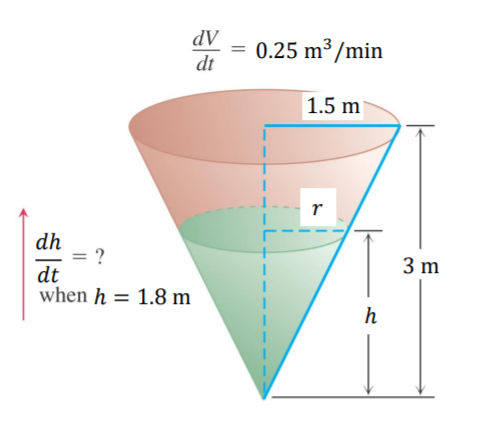
\includegraphics[width = 0.4\linewidth]{Images/ex1 chain rule.png}
    \caption{Illustration of example 1}
\end{figure}

\paragraph{Answer :}
First we have 
\[
    V = \frac{1}{3} \pi r^2 h
\]

\noindent 
From the figure we can see that the ratio of $r$ and $h$ is :
\begin{align*} 
    \frac{r}{h} &= \frac{1.5}{3} = \frac{1}{2} \\
    r &= \frac{1}{2} h 
\end{align*}
    
So, we have
\begin{align*} 
     V &= \frac{1}{3} \pi \left( \frac{1}{2} h \right)^2 h \\
     V &= \frac{1}{12} \pi h^3 \\
     \frac{dV}{dh} &= \frac{3}{12} \pi h^2 = \frac{1}{4} \pi h^2
\end{align*}

Then,
\begin{align*} 
    \frac{dV}{dt} &= \frac{dV}{dh} \cdot \frac{dh}{dt} \\
    \frac{dh}{dt} &= \frac{\frac{dV}{dt}}{\frac{dV}{dh}} \\
     &= \frac{0.25}{\frac{1}{4} \pi \cdot (1.8)^2} \\
     &= \frac{25}{81 \pi}\: m/min
\end{align*}

\paragraph{Example 2}
A particle P moves clockwise at a constant rate along a circle of radius
10 m centered at the origin. The particle’s initial position is (0, 10) on the y-axis, and its
final destination is the point (10, 0) on the x-axis. Once the particle is in motion, the tangent
line at P intersects the x-axis at a point Q (which moves over time). If it takes the
particle 30 s to travel from start to finish, how fast is the point Q moving along the x-axis
when it is 20 m from the center of the circle?

\begin{figure}[h!] 
    \centering
    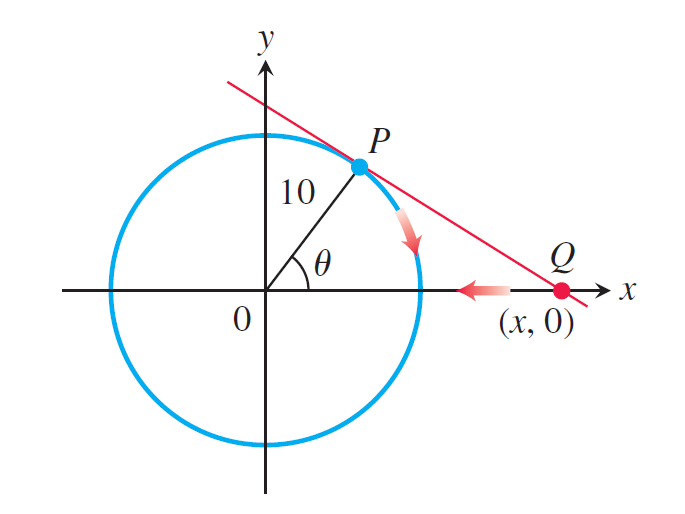
\includegraphics[width = 0.4\linewidth]{Images/ex2 chain rule.png}
    \caption{Illustration of example 2}
\end{figure}

\paragraph{Answer :} From the graph we can see that
\begin{align*} 
    \cos \theta &= \frac{10}{x} \\
    \frac{d}{d\theta} \cos \theta &= \frac{d}{d\theta} \frac{10}{x} \\
    - \sin \theta &= - \frac{10}{x^2} \cdot \frac{dx}{d\theta} \\
    \frac{dx}{d\theta} &= \frac{\sin \theta \cdot x^2}{10} \\
    &= \frac{\sqrt{x^2 - 100}\cdot x}{10}  
\end{align*}

And we also have,
\begin{align*} 
    \frac{\pi}{2} &= \frac{d\theta}{dt} \cdot 30 \\
    \frac{d\theta}{dt} &= (-) \frac{\pi}{60} \\
\end{align*}

So,
\begin{align*} 
     \frac{dx}{dt} &= \frac{dx}{d\theta} \cdot \frac{d\theta}{dt} \\ 
     &= \frac{\sin \theta \cdot x^2}{10} \cdot - \frac{\pi}{60} \\
     &= - \frac{\sqrt{20^2 - 100} \cdot 20}{10} \cdot \frac{\pi}{60} \\
     &= - \frac{200 \sqrt{3}}{10} \cdot \frac{\pi}{60} \\ 
     &= - \frac{1}{3} \pi \sqrt{3}\; m/s
\end{align*}

\section{Implicit Differentiation}
\subsection{Implicitly vs Explicitly Defined Equation}
Explicitly defined function is a function that is defined clearly in the form of $y = ...x$. On the other hand, Implicitly
defined function is a function that is expressed by an implicit equation that relates one variable to another. \\
For example: $y = \sqrt{1 - x^2}$ is defined explicitly, $x^2 + y^2 = 1$ is defined implicitly.
\subsection{Implicit Differentiation}
Let an equation defined as:
\[
    x^2 + y^2 = 1
\]
What is slope of the tangent line at $(1/\sqrt{2}, 1/\sqrt{2})$?

There are two ways to solve the problem. First, explicit differentiation, that is we modify the equation to be an 
explicitly defined function.

\begin{align*} 
    x^2 + y^2 &= 1 \\
    y^2 &= 1 - x^2 \\ 
    y &= \pm \sqrt{1 - x^2}
\end{align*}

Because $y = 1/\sqrt{2} > 0$, then $y = \sqrt{1 - x^2}$.
Hence,
\begin{align*} 
    \frac{dy}{dx} &= \frac{1}{2 \sqrt{1 - x^2}} \cdot ( - 2x)\\
    &= \frac{ - x}{\sqrt{1 - x^2}} \\
    \left. \frac{dy}{dx} \right|_{x = \frac{1}{\sqrt{2}}} &=  \frac{ - \frac{1}{\sqrt{2}}}{\sqrt{1 - \frac{1}{2}}} = - 1
\end{align*}

The next method is by implicit differentiation:
\begin{enumerate} 
    \item Differentiate both sides of the equation with respect to $x$, treating $y$ as a differentiable
    function (using chain rule)
    \item Collect the terms with $dy/dx$ on one side of the equation and solve for $dy/dx$
\end{enumerate}

\begin{align*} 
    x^2 + y^2 &= 1 \\
    2x + 2y \cdot \frac{dy}{dx} &= 0 \\
    2y \cdot \frac{dy}{dx} = - 2x \\
    \frac{dy}{dx} = \frac{ -x}{y} \\
    \left. \frac{dy}{dx} \right|_{x = \frac{1}{\sqrt{2}}} &= \frac{ - \frac{1}{\sqrt{2}}}{\frac{1}{\sqrt{2}}} = - 1 
\end{align*} 

\subsection{Exception}
Implicit differentiation can only be used if:
\begin{itemize} 
     \item Function doesn't have vertical tangent at the specific point
     \item $y$ can be defined as function of $x$ locally around the specific point 
\end{itemize}

\paragraph{Example} Let an equation defined as
\[
    x^3 + y^3 - 6xy = 0
\]

At $(0,0)$, we can't find the derivative using implicit differentiation because it can't be defined as a function of $x$, and
have a vertical tangent. However, at $(x,y) = (3,3)$, for instance, we can find the derivative:
\begin{align*} 
     x^3 + y^3 - 6xy &= 0 \\
     3x^2 + 3y^2 \cdot \frac{dy}{dx} - (6x \cdot \frac{dy}{dx} + 6y) &= 0 \\
     3x^2 - 6y &= (6x - 2y) \cdot \frac{dy}{dx} \\
     \frac{dy}{dx} &= \frac{3x^2 - 6y}{6x - 3y^2} \\
     \left. \frac{dy}{dx} \right|_{(x,y) = (3,3)} &= \frac{3(3)^2 - 6(3)}{6(3) - 3(3)^2} = - 1
\end{align*}

\subsection{Normal Line}
For the graph of a differentiable function $y = f(x)$, normal line is a line that is perpendicular
with the tangent line. The slope of the normal line at $(x_0, y_0)$ is 
\[
    m_{normal} = \frac{ -1}{f'(x)}
\] 
Provided that $f'(x) \neq 0$

\paragraph{Example} From example in 7.3, find the normal and tangent line of the graph at (3,3) \\
\\ 
\begin{figure}[h!] 
    \centering
    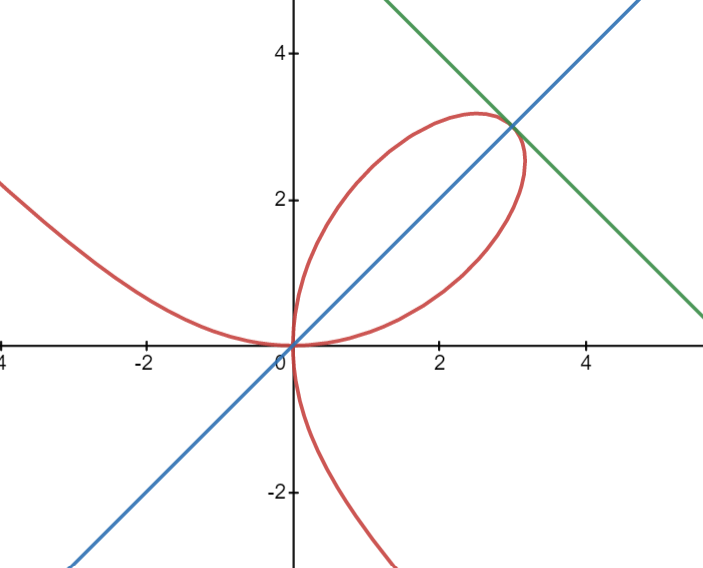
\includegraphics[width= 0.3\linewidth]{Images/normal line.png}
    \caption{Graph of $x^3 + y^3 -6xy = 0$, at $(0,0)$ it has vertical tangent. 
    Blue line is the normal line, and the green line is the tangent line.}
\end{figure}
\textbf{Tangent Line: } 
\begin{align*} 
    y - 3 &= - 1(x - 3) \\
    y &= - x + 6
\end{align*}

\noindent
\textbf{Normal Line: }
\begin{align*} 
    y - 3 &= \left(\frac{ - 1}{m_{tangent}} \right) (x - 3) \\
    y - 3 &= \left(\frac{ -1}{ - 1} \right) (x - 3) \\
    y - 3 &= 1(x - 3) \\
    y &= x
\end{align*}

\section{Linearization}
\subsection{Linear Approximation}
Suppose we want to compute $f(x)$ for any $x \in (a - \delta , a + \delta)$, with $\delta$ close to 0. 
We may replace $f(x)$ with a linear function, which only provides approximation.

\paragraph{Definition}
If $f$ is differetiable at $a$, for $x$ "near" $a$ we have
\[
    \frac{f(x) - f(a)}{x - a} \approx f'(a) 
\]
In other words,
\[
    \textrm{Slope of secant on the interval } [a - \delta, a + \delta] \approx\,\textrm{Slope of tangent line at } a
\]

\noindent
So, we have
\[
    L_a(x) = f(a) + f'(a) \cdot (x - a)
\]
with 
\[
    L_a(x) \approx f(x)
\]
L is the standard linear approximation of $f$ at $a$ with $x = a$ as the center of approximation.

\begin{figure}[h!]
     \centering
     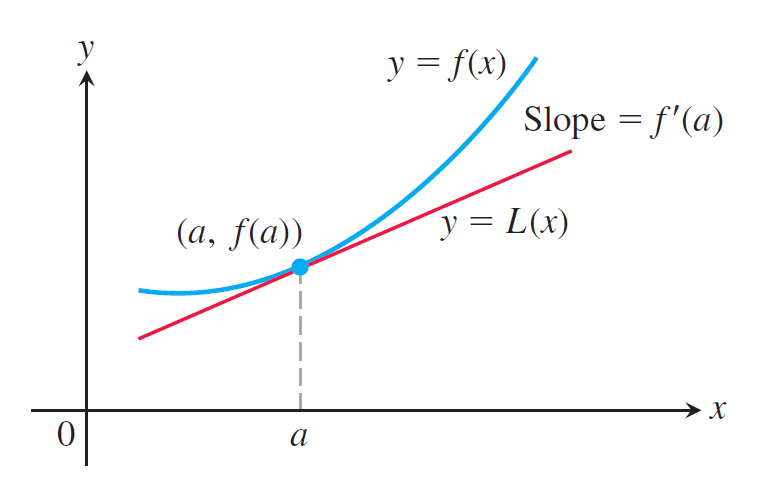
\includegraphics[width=0.5\linewidth]{Images/linearization.png}
     \caption{The tangent to the curve $y = f(x)$ at $a$ is $L(x)$}
\end{figure}
\paragraph{Example 1}
Approximate the numerical value of $\sqrt[3]{27.4}$ by considering linearization of $f(x) = \sqrt[3]{x}$ centered at $x = 27$

First,
\begin{align*} 
     f(27) &= \sqrt[3]{27} = 3 \\
\end{align*}

Then,
\begin{align*} 
    f'(x) &= \frac{1}{3x^{\frac{2}{3}}} \\
    f'(27) &= \frac{1}{3(9)} = \frac{1}{27} \\
\end{align*}

So,
\begin{align*} 
    L_{27}(x) &= f(27) + f'(27) \cdot (x - 27) \\
    &= 3 + \frac{1}{27} \cdot (x - 27) \\
    &= 2 + \frac{x}{27} \\
    L_{27}(27.4) &= 2 + \frac{27.4}{27} \approx 3.0148148
\end{align*}

\paragraph{Example 2} 
Approximate $(1 + \epsilon)^k$ for small $\epsilon$! \\ \\

We have $f(x) = x^k$, we need to approximate $f(x)$ centered at $x = 1$. First:
\[
    f'(x) = kx^{k - 1} \Rightarrow f'(1) = k
\]

Hence,
\begin{align*} 
    L_1{\epsilon} &= f(1) + f'(1)(\epsilon) \\
    &= 1 + k\epsilon \\
    f(1 + \epsilon) &\approx 1 + k\epsilon
\end{align*}
\subsection{Differential}
Sometimes we use the Leibniz notation $dy/dx$ to represent the derivative of $y$ with respect
to $x$. However, it is not actually a ratio.

\paragraph{Definition}
Let $y = f(x)$ be a differentiable function. The differential $dx$ is an
independent variable. The differential $dy$ is 
\[
    dy = f'(x) dx
\]

$dy$ depends on the value of $dx$ and $x$. We call $dy$ and $dx$ as \textbf{differential}. They are infinitesmall, that is 
a "tiny tiny bit" of $x$ and $y$ or a very small value of $x$ and $y$.

\paragraph{Example} 
For $y = f(x) = x^5 +37x$, when $x = x_0 = 1$ and $dx = 0.2$, then 
\begin{align*} 
    dy = f'(x) dx = (5x^4 + 27) |_{x = 1}\:  (0.2) = 8.4
\end{align*}

\paragraph{Linearization using differentials} Consider $L(x)$
\begin{figure} 
    \centering
    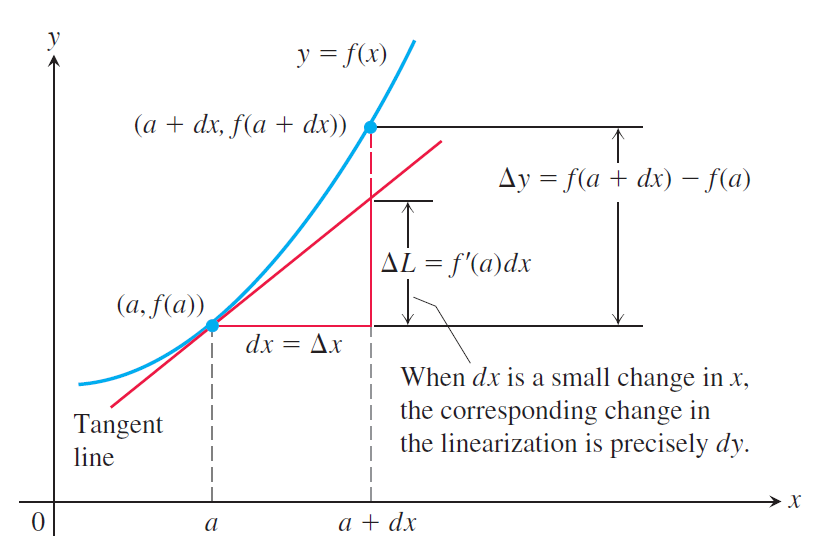
\includegraphics[width = 0.5\linewidth]{Images/differentials.png}
    \caption{$\Delta L = dy$, $dy - \Delta y$ is the difference of the actual function with the linear approximation (tangent line)}
\end{figure}

\begin{align*} 
     L(x_0 + dx) &= f(x_0) + f'(x_0) (x_0 + dx - x_0) \\
     L(x_0 + dx) &= f(x_0) + f'(x_0) (dx) \\
     f'(x_0) (dx) &= L(x_0 + dx) - f(x_0) \\
     dy &= L(x_0 + dx) - f(x_0) 
\end{align*}

\noindent
Hence, standard linear approximation of $f(x_0 + \Delta x)$ centered at $x = x_0$ :
\[
    f(x_0 + dx) \approx L(x_0 + dx) = f(x_0) + dy
\]

\paragraph{Example} If the radius of a circle increases from 10 m to 10.1 m, then its change of area can be approximated:
\[
    A = f(r) = \pi r^2 \textrm{ \tab and \tab } dr = 0.1m
\]

\begin{align*} 
     f(10.1) \approx f(10) + dA &= f(10) + f'(10) dr \\
     &= \pi \cdot 10^2 + 2 \pi \cdot 10 \cdot 0.1 \\
     &= 100\pi + 2\pi = 102\pi 
\end{align*}

\paragraph{Sensitivity of Change}
The equation $dy = df = f'(x)$ measures how sensitive the output $f$ is to a small change in $x$-value.
The larger the value of $f'$ at $x$, the greater the effect of a given change $dx$.

\begin{figure}[h!]
    \centering
    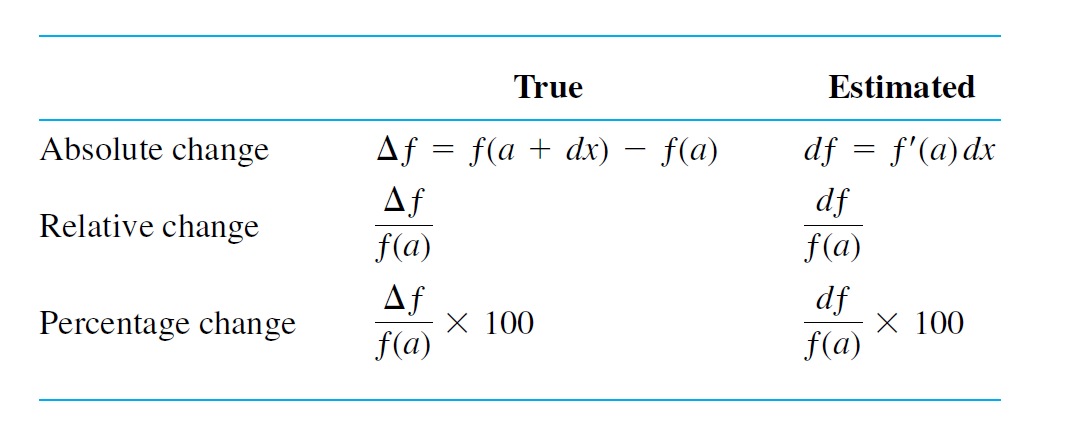
\includegraphics[width = 0.6\linewidth]{Images/sensitivity.png}
    \caption{How we describe the sensitivity of change}
\end{figure}

\paragraph{Example}
An object falls such that its position from the starting point is given by $s = 4.9x^2$. Time measurement may have an error of $\pm 0.01 s$.
So, the error of distance measured is:
\begin{align*} 
     ds = s'(t)dt = 9.8t \cdot dt = \pm 0.098 t
\end{align*}

\subsection{Error of Approximation}
We know that the linear approximation of $f(x)$ centered at $x = a$ is 
\[
    L(x_0 + \Delta x) = f(x_0) + f'(x_0)(\Delta x)
\]
But what is the error of the approximation, that is 
\[
    f(x_0 + \Delta x) - L(x_0 + \Delta x) = ?
\]

\noindent
First, from the definition
\begin{align*} 
     f(x_0 + \Delta x) - L(x_0 + \Delta x) &= f(x_0 + \Delta x) - f(x_0) - f'(x_0) \Delta x \\
     &= \left(\frac{ f(x_0 + \Delta x) - f(x_0)}{\Delta x} - f'(x_0) \right) \Delta x
\end{align*}

\noindent
Let $\epsilon = \left(\frac{ f(x_0 + \Delta x) - f(x_0)}{\Delta x} - f'(x_0) \right)$
with $\frac{ f(x_0 + \Delta x) - f(x_0)}{\Delta x}$ as the slope of secant line, and $f'(x_0)$ as the slope of tangent line. So,
\begin{align*} 
    f(x_0 + \Delta x) - L(x_0 + \Delta x) &= \epsilon \Delta x
\end{align*}

\noindent
Since, $\epsilon = \left(\frac{ f(x_0 + \Delta x) - f(x_0)}{\Delta x} - f'(x_0) \right)$, we have
\begin{align*} 
    \lim_{\Delta x \to 0} \epsilon = \lim_{\Delta x \to 0} \frac{ f(x_0 + \Delta x) - f(x_0)}{\Delta x} - f'(x_0) = 0
\end{align*}

\noindent
Then, 
\begin{align*} 
    f(x_0 + \Delta x) - L(x_0 + \Delta x) &= \epsilon \Delta x \\
    \frac{f(x_0 + \Delta x) - L(x_0 + \Delta x)}{\Delta x} &= \epsilon \\
    \lim_{\Delta x \to 0} \frac{f(x_0 + \Delta x) - L(x_0 + \Delta x)}{\Delta x} &= \lim_{\Delta x \to 0} \epsilon = 0
\end{align*}

That means, as $\Delta x$ become smaller and smaller, the error decreases approaching 0.

\paragraph{Definition}
If $y = f(x)$ is differentiable at $x = a$ and $x$ changes from $a$ to $a + \Delta x$, the
change $\Delta y$ in $f$ is given by
\[
    \Delta y = f'(a)\Delta x + \epsilon \Delta x
\]
with $\Delta y$ as the true changes, $f'(a)\Delta x = dy$ as the estimate changes, and $\epsilon \Delta x$ as the error of approximation.

\subsection{Proof of Chain Rule}
We want to show that $(g \circ f)'(x_0) = g'(f(x_0))f'(x_0)$.\\
First, let $y = f(x)$, $z = g(y) = g(f(x))$. \\ 

\noindent
Suppose $x$ changes by $\Delta x$. Let $\Delta y$ and $\Delta z$ is corresponding to the changes to $y$ and $z$ respectively.
Then, 
\[
    \Delta y = f'(x_0) \Delta x + \epsilon_1 \Delta x \textrm{ for some } \epsilon_1 \textrm{ with }\lim_{\Delta x \to 0} \epsilon_1 = 0
\]

\[
    \Delta z = g'(y_0) \Delta y + \epsilon_1 \Delta y \textrm{ for some } \epsilon_2 \textrm{ with }\lim_{\Delta y \to 0} \epsilon_2 = 0
\]

So,
\begin{align*} 
    \frac{\Delta z}{\Delta x}  &= g'(y_0) \frac{\Delta y}{\Delta x}  + \epsilon_2 \frac{\Delta y}{\Delta x} \\
    &= g'(y_0) \frac{f'(x_0) \Delta x + \epsilon_1 \Delta x}{\Delta x}  + \epsilon_2 \frac{f'(x_0) \Delta x + \epsilon_1 \Delta x}{\Delta x} \\
    &= (g'(y_0) + \epsilon_2)(f'(x_0) + \epsilon_1) \\
\end{align*}

As $\Delta x \to 0$, $\epsilon_1, \epsilon_2 \to 0$, So
\begin{align*} 
    \lim_{\Delta x \to 0}\frac{\Delta z}{\Delta x} &= g'(y_0)f'(x_0) \\
    \frac{dz}{dx} &= g'(f(x_0)f'(x_0) 
\end{align*}

\end{document}